\section{Introduction}\label{sec:Introduction}

In this note we present the analysis for the total inclusive negatively charged pion-Argon ($\pi^{-}$-Ar) interaction cross-section for LArIAT data collected over Run-I and Run-II. The note is broken into four section: Section \ref{sec:Introduction} gives an introduction to $\pi$ interaction cross-sections and the LArIAT beamline, Section \ref{sec:DataSamples} provides an introduction to the data and Monte Carlo samples used in this analysis along with preliminary selection cuts to pre-select a sample of $\pi, \mu, e$ candidates. Section \ref{sec:PionAnalysis} provides an overview of the inclusive $\pi$ cross-section analysis and the ``thin slice'' method for measuring the kinetic energy, finally Section \ref{sec:Results} gives the results for the analysis.

%%%%%%%%%%%%%%%%%%%%%%%%%%%%%%%%%%%%%%%%%%%%%%%%%%%%%%%%%%%%%%%%%%%%%%%%%%%%%%%%%
\subsection{Pion Interaction Cross-Section}\label{sec:PiCrossSection}
%%%%%%%%%%%%%%%%%%%%%%%%%%%%%%%%%%%%%%%%%%%%%%%%%%%%%%%%%%%%%%%%%%%%%%%%%%%%%%%%%
Pion interactions with matter have been a central topic in particle physics for decades. Over the past forty years, an extensive set of pion scattering experiments have been conducted at various meson factories. Although this data has provided detailed measurements of differential cross sections for a variety of final state kinematic variables, the uncertainties on the total pion cross sections range from 10-30\% for light nuclei, and even larger for heavy nuclei.

The total $\pi^{-}$-Ar interaction cross-section measured in this analysis can be defined as:

\begin{equation}
\sigma_{tot}= \sigma_{el}+\sigma_{reac}\\
\end{equation}
where $\sigma_{el}$ is the elastic scattering component of the cross-section and $\sigma_{reac}$ represents the remaining `reaction' cross-section

\begin{equation}
\sigma_{reac}=\sigma_{inel}+\sigma_{abs}+\sigma_{chex}+\sigma_{\pi prod},
\end{equation}
including in-elastic ($\sigma_{inel}$), absorption ($\sigma_{abs}$), charge-exchange ($\sigma_{chex}$), and pion-production ($\sigma_{\pi prod}$). These interactions are the strong interactions related to a single hadronic process.

Experimental data for $\pi$-Ar interactions is sparse and current MC simulations, such as Geant4, interpolate interaction models for argon based upon data from lighter and heavier nuclei.  Figure \ref{fig:Geant4CrossSection} from DocDB-1923 shows the expected $\pi$-Argon cross-section broken down by the total, inelastic, and elastic components over the kinetic energy range between 0-2000~MeV.

\begin{figure}[ht!]
\centering
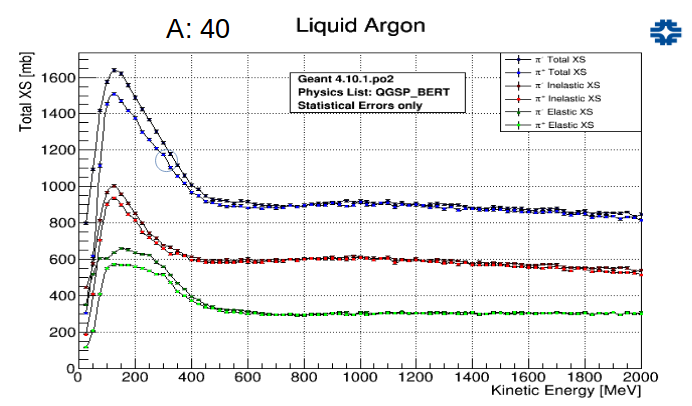
\includegraphics[scale=0.45]{./images/ArgonPionCrossSection.png}\\
\caption{$\pi$-Argon interaction cross-section generated using Geant4 (v4.10.1.po2) using the QGSP BERT model over the relevant kinetic energy range for LArIAT. See DocDB-1923 for more details.}
\label{fig:Geant4CrossSection}
\end{figure}

The pion interaction cross section depends on the mass of the target nucleus, as shown in Figure \ref{fig:Adep}, for different interaction channels near the $\Delta$-resonance region.

 
\begin{figure}[ht!]
\centering
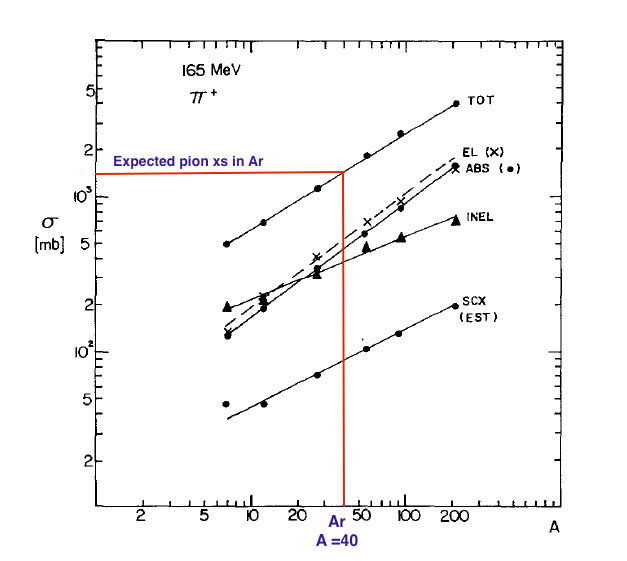
\includegraphics[scale=0.45]{./images/pionXS_vs_A.png}\\
\caption{Nuclear mass (A) dependence of $\pi^{+}$-nucleus interaction cross section for different interaction channels nearby the $\Delta$ resonance-region for 165 MeV/c pions.\cite{ashery1}}
\label{fig:Adep}
\end{figure}

Beyond intrinsic theoretical interest in nuclear structure, pion interactions play a critical role in understanding systematic uncertainties in neutrino experiments conducted at the GeV energy scale. Charged pions are produced in noticeable numbers in neutrino interactions with nuclei for neutrino energies of a few GeV.  

The interaction cross section of the pion strongly affects the possibility of detecting and measuring the pions. When pions are produced in $\nu$-Ar interactions, the inferred neutrino energy is based upon the measurement of the pion energies. Since the predicted pion cross section for interactions with nuclei is large, especially near the $\Delta$ resonance energy region, pion cross-sections can strongly impact the neutrino oscillation measurement. Thus, the precise measurement of the $\pi$-Ar interaction cross-section is important to future liquid argon neutrino experiments. In particular, current (MicroBooNE) and future (SBN and DUNE) neutrino oscillation experiments are very sensitive to pion cross section uncertainties. 

%%%%%%%%%%%%%%%%%%%%%%%%%%%%%%%%%%%%%%%%%%%%%%%%%%%%%%%%%
\subsection{Overview of the LArIAT Beamline}\label{sec:beamline}
%%%%%%%%%%%%%%%%%%%%%%%%%%%%%%%%%%%%%%%%%%%%%%%%%%%%%%%%%
The LArIAT experiment takes place at the Fermilab Test Beam Facility (FTBF) located in the Meson Building at Fermilab. A beam of 120~GeV protons is transported to the Meson Building and split to make two beam lines known as MCenter and MTest. LArIAT is served by the MCenter beam line, whose primary beam of 120~GeV protons impinges upon a thick target (25~cm) to create a secondary beam of charged particles, mainly pions, 8 - 80 GeV range. This collimated pion beam is momentum-selected and then transported the MC7 radiation enclosure, the LArIAT experiment hall.  

In the MC7 enclosure the secondary beam focuses onto a thick copper target and the resulting tertiary beam is collimated by a 1~m iron shield with an opening $-13\deg$ to beam's right with respect to the secondary beam direction. Two analyzing dipole magnets steer the beam path $+10\deg$, selecting a momentum window within 0.2 and 2.0~GeV/c and sign-selecting the particles and steering them to the TPC. The tertiary beam is instrumented with a pair of Time-of-Flight (TOF) scintillating detectors,  four Wire Chambers (WC) which allow measurement of each particle's momentum based on the location of the hits in the wire chambers, two Aerogel Cherenkov counters (AG) of different Cherenkov threshold to allow for $\mu / \pi$ separation, the LArTPC detector and a Muon Range Stack. Figure \ref{fig:beamlineschematic} gives a diagram of the tertiary beam line within the MC7 enclosure.

\begin{figure}[htb]
\begin{center}
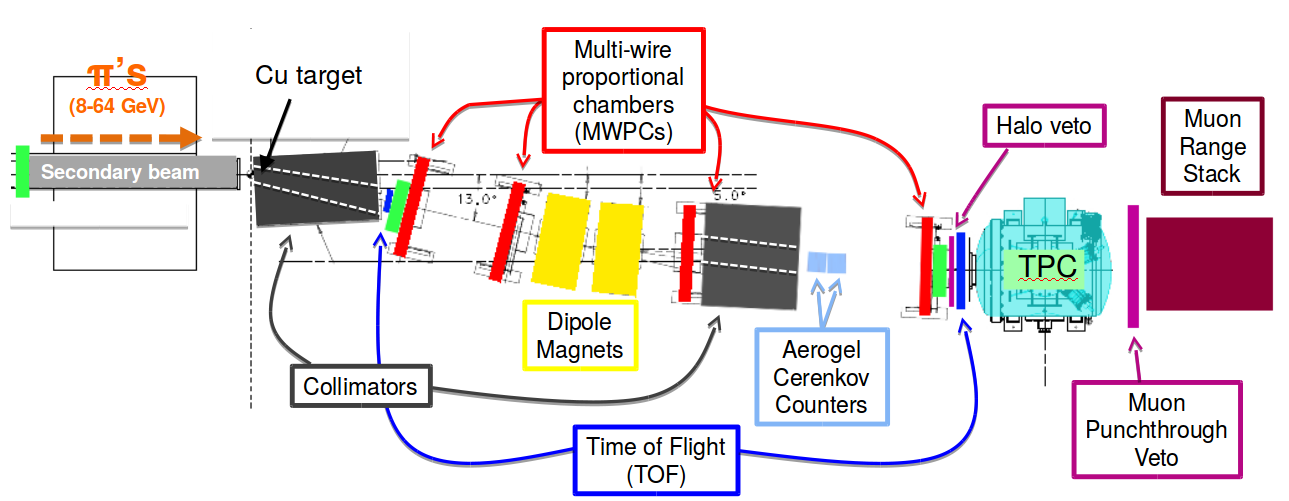
\includegraphics[scale=0.25]{./images/mc7beamline.png}
\end{center}
\caption{Schematic of the Tertiary Beam line within the MC7 enclosure.}
\label{fig:beamlineschematic}
\end{figure}

In this analysis, only the information from the Wire Chambers and the Time-of-Flight is used for particle identification. In particular, it is possible to calculate the mass of a given beamline track using the following equation

\begin{equation}
mass = \frac{p}{c}\sqrt{(\frac{TOF \times c}{l})^2 -1}
\end{equation}
where $p$ represents the measured momentum from the wire chamber, $TOF$ represents the time-of-flight measured as the difference between the two time-of-flight paddles in the LArIAT beamline, $l$ is path length the particle traveled down the beamline, and $c$ represents the speed of light. As is outlined in Section \ref{sec:EventSelection}, this allows us to select events based on the particle species.

%%%%%%%%%%%%%%%%%%%%%%%%%%%%%%%%%%%%%%%%%%%%%%%%%%%%%%%%%%%%%%%%%%%%%%%%%
\subsection{Beam composition}\label{sec:G4BeamlineMC}
%%%%%%%%%%%%%%%%%%%%%%%%%%%%%%%%%%%%%%%%%%%%%%%%%%%%%%%%%%%%%%%%%%%%%%%%%
The tertiary beam composition depends upon the energy of the secondary beam and the choice of magnetic field in the analyzing magnets. In Table \ref{tab:beamcomp1} and Table \ref{tab:beamcomp2} the beam composition is given in terms of percentage of different particle species per spill for negative and positive polarity. These are averaged values on several primary beam energies and magnets field intensities from MC simulations of the tertiary beam. As an example, the tertiary beam particle species and energy spectra for and negative polarity Monte Carlo and Data is shown in Figure \ref{fig:beamspectrum}  with 64 GeV of energy and the magnet setting of -100 T.

\begin{table}[ht!]
\centering
\begin{tabular}{|l|l|l|l|l|l|l|}
\hline
                      & $\pi^-$ & $e^-$ & $\gamma$ & $\mu^-$ & $K^-$ & $\overline{p}$ \\ \hline
Beam Composition (\%) &   48.4      &   40.9    &     8.5     &    2.2     &      0.035  &     0.007           \\ \hline
\end{tabular}
\caption{Beam Composition - Negative polarity configuration (from MC)}
\label{tab:beamcomp1}
\end{table}


\begin{table}[ht!]
\centering
\begin{tabular}{|l|l|l|l|l|l|l|}
\hline
                   & $\pi^+$ & $e^+$ & $\gamma$ & $\mu^+$ & $K^+$ & p \\ \hline
Beam Composition (\%) &    42.8     &  30.1     &    8.6      &    2.1     &    0.057    &    16.2            \\ \hline
\end{tabular}
\caption{Beam Composition - Positive polarity configuration (from MC)}
\label{tab:beamcomp2}
\end{table}



\begin{figure}[htb]
\begin{center}
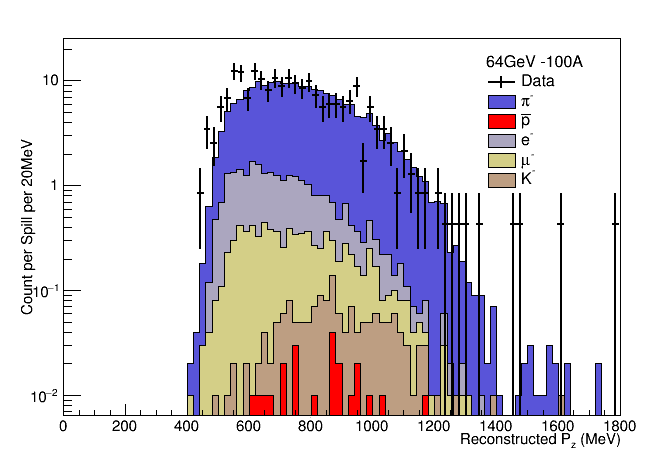
\includegraphics[scale=0.45]{./images/BeamSpectrumExample.png}
\end{center}
\caption{Tertiary Beam spectra for negative 100 Amp, 64 GeV target energy (from MC) with data overlayed.}
\label{fig:beamspectrum}
\end{figure}
